\setcounter{chapter}{2}
\chapter{Circuiti Elettrici}

\section{Condensatori}

In generale un condensatore \`e una coppia di conduttori che hanno carica Q e -Q rispettivamente. Un  esempio \`e dato da due piani conduttori in parallelo.

\subsection{Condensatore a piani paralleli}

\begin{wrapfigure}{r}{0.4\textwidth} % 'r' for right, 'l' for left
    \centering
    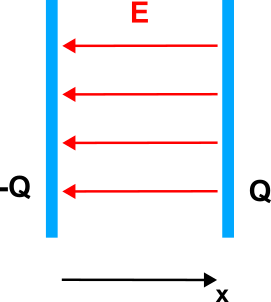
\includegraphics[width=0.3\textwidth]{images/parallelcapac} % Replace with your image
\end{wrapfigure}
Consideriamo due piani conduttori posti in parallelo come in figura, e assumiamo che la distanza $d$ tra i piani sia molto pi\`u piccola di $\sqrt{A}$ dove $A$ \`e l'area delle superfici planari. Imporre una condizione del genere ci permette di considerare gli effetti che si generano al bordo dei piatti e quindi possiamo assumere che il campo elettrico che generato nella regione tra i due piani coincide con quello che si avrebbe se le superfici avessero una estensione infinita. Il campo elettrico \`e dato da 
\begin{equation*}
	\bold{E} = -\frac{\sigma}{\varepsilon_0} \bold{\hat{x}}
\end{equation*}
dove $\sigma = Q/A$ e il campo ha direzione opposta a quella dell'asse $x$. Definiamo \textit{capacitanza} la grandezza 
\begin{equation}
	C = \frac{Q}{V}
\end{equation}
dove V rappresenta il $voltaggio$ o la \textit{differenza di potenziale}, tra i due piani paralleli. Dato che $\bold{E} = -\frac{d\phi}{dx}$, avremo che 
\begin{equation*}
	\phi(x) =-Ex+c \quad \Rightarrow \quad V = \phi(0) - \phi(d) = Ed = \frac{Qd}{A \varepsilon_0}
\end{equation*} 
e  quindi possiamo concludere che la capacitanza per due piatti paralleli di area A e posti ad una distanza $d$, sono
\begin{equation*}
	C = \frac{A \varepsilon_0}{d}
\end{equation*}
La capacitanza di un condensatore dipende dalla sua geometria e non dalla carica Q. I condensatori in generale vengo usati per immagazzinare energia elettrica. L'energia accumulabile da un condensatore \`e data dalla relazione 
\begin{equation*}
	U = \frac{1}{2} \varepsilon_0 \int_V dV \; \bold{E} \cdot \bold{E} = \frac{A \varepsilon_0}{2} \int_{0}^{d} dx \; \left ( \frac{\sigma}{\varepsilon_0}\right)^2 = \frac{Q^2}{2C}
\end{equation*}
L'unit\`a di misura per la capacitanza \`e data dal \textit{Farad} che \`e dato da 
\begin{equation*}
	[F] = \frac{[Coulomb]}{[Volt]}
\end{equation*}
Poich\`e la capacit\`a dei conduttori isolati ( e dei condensatori) sono proporzionali a $\varepsilon_0$ tramite una lunghezza (parametro di scala), torna utilie esprimere $\varepsilon_0$ in unit\`a di capacit\`a per unit\`a di lunghezza
\begin{equation*}
	\varepsilon_0 = 8,8 \times 10^{-12} \frac{F}{m}
\end{equation*}


Il condensatore planare che si \`e "ideale", ovvero \`e una trattazione semplificata che non tiene conto di alcune caratteristiche come gli effetti di bordo del campo elettrico che viene ipotizzato essere completamente contenuto all'interno del volume racchiuso tra le armature; 
\begin{wrapfigure}{l}{0.4\textwidth}
  \centering
  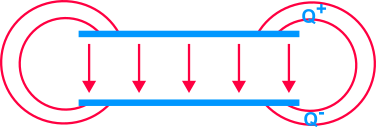
\includegraphics[width=0.38\textwidth]{images/edge_effect}
\end{wrapfigure}
questa semplificazione risulta essere pertinente con la realt\`a se la distanza tra i piatti $d \ll \sqrt{A}$ alla loro area o raggio se sono di natura circolare. 
\textit{In un disco conduttore isolato la distribuzione di carica $\sigma$ non \`e uniforme}, ma in una coppia di dischi ideali s\`i.
\newpage

\subsection{Conduttori con condensatore interno e esterno}

\begin{wrapfigure}{r}{0.4\textwidth}
  \centering
  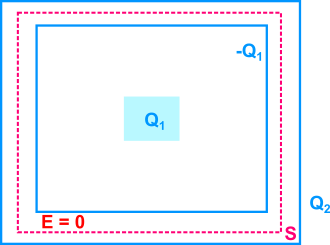
\includegraphics[width=0.38\textwidth]{images/cond_cons}
\end{wrapfigure}
Esempi di conduttori con all'interno condensatori sono i cavi coassiali. Per definizione la capacit\`a di un condensatore \`e data da 
\begin{equation*}
	C = \frac{Q_1}{\phi_1 - \phi_2}
\end{equation*}
dato che il campo nella cavit\`a dipende solo dalla carica $Q_1$. Per definizione il campo all'interno di un conduttore \`e nullo $\bold{E} = 0$ e di conseguenza anche il suo flusso $\phi_{S}(\bold{E}) = 0$, si ha dunque \textit{induzione completa}. Un eventuale carica $Q_2$ si distribuisce sulla superficie esterna. Possiamo vedere il sistema come due sotto sistemi uno costituito solo da $Q_1$ e uno costituito da $Q_2$ usando il principio di sovrapposizione di ottiene in il sistema di partenza. Il sistema che possiede solo $Q_2$ ha $\bold{E} =0$ all'interno della cavit\`a e dunque $Q_2$ \`e solo esterna. Il fatto che internamente il campo sia nullo nella configurazione in cui \`e presente solo $Q_2$, fa s\`i che il potenziale internamente sia costane 
\begin{equation*}
	\bold{E}_2 = - \nabla\phi_2 = 0 \Rightarrow \phi_2 = \text{cost}
\end{equation*}
di conseguenza nel sistema complessivo la differenza di potenziale dipende solo dal campo interno
\begin{equation*}
	\phi_{1} - \phi_2 = \int_{1}^{2} \bold{E}_{int} \cdot d\bold{s}
\end{equation*}
lungo un qualunque percorso tra i conduttori. Notare che $\phi_{2}$ \`e fissato dalle condizioni al contorno date dalla geometria della superficie esterna del conduttore.

\subsubsection{Esempio: Condensatore cilindrico}

Consideriamo un sistema formato da una distribuzione di carica lineare $\lambda = Q/L$ distribuita su un cilindro di raggio a, questo \`e racchiuso da un superficie cilindrica conduttrice di raggio b, dove $b>a$. Il campo elettrico interno \`e dato da 
\begin{equation*}
	E_{int} = \frac{\lambda}{2 \pi \varepsilon_0 } \frac{1}{r } \quad r \in [a,b]
\end{equation*}
e la differenza di potenziale \`e 
\begin{equation*}
	\varphi(a) - \varphi(b) = \int_{a}^{b} \bold{E} \cdot d\bold{s} = \frac{Q}{2 \pi \varepsilon_0 L } \log \left(\frac{b}{a}\right )
\end{equation*}
di conseguenza la capacit\`a \`e data da
\begin{equation*}
	C = \frac{Q}{\Delta \phi} = \frac{2 \pi \varepsilon_0 L}{\log \left(\frac{b}{a} \right)}
\end{equation*}

\subsection{Sistemi di conduttori (o condensatori a pi\`u strati)}

Consideriamo un sistema formato da N conduttori, per il quale ad infinito il potenziale vale $\phi = 0$. Prendiamo in analisi un singolo conduttore su cui \`e presente una carica $Q_i$, siccome un conduttore carico non interagisce con se stesso, la sua distribuzione di carica \`e legata al campo elettrico degli altri conduttori presenti nel sistema. Ovvero
\begin{equation*}
	\bold{E} = \sum_{i = 1}^{N-1}\bold{E}_i
\end{equation*} 
per il principio di sovrapposizione, la carica del condensatore \`e legata al campo dall Legge di Gauss dove 
\begin{equation*}
	\int_{S} \bold{E} \cdot d\bold{a} = \frac{Q_i}{\varepsilon_0} = \frac{1}{\varepsilon_0}\int_{V} \rho d\nu
\end{equation*}
utilizzando il teorema della divergenza si ha che 
\begin{equation*}
	\int_{S} \bold{E} \cdot d\bold{a}=\int_{V} (\nabla \cdot \bold{E}) \cdot d\nu
\end{equation*}
e dunque 
\begin{equation*}
	\nabla \cdot \bold{E} = \frac{\rho}{\varepsilon_0}
\end{equation*}
Dato che degli altri conduttori nel sistema conosciamo il potenziale possiamo esprimere la divergenza del campo elettrico, nell'equazione di Poisson 
\begin{equation*}
	\nabla^2\phi = - \frac{\rho}{\varepsilon_0}
\end{equation*}
dove ovviamente $\phi$ \`e il poteziale totale associato al campo $\bold{E}$. Per il teorema di unciti\`a la soluzione dell'equazione di Poisson \`e unica e questo ci garantisce che la carica sull'i-esimo conduttore \`e identificata in modo univoco.